\begin{frame}
    \centering
    \begin{figure}[H]
        
\includegraphics[keepaspectratio, width=0.7\paperwidth, height=\paperheight]{LeeLogo}
    \end{figure}
    Informatik: Programmieren\\
    Lektion 08 \emoji{alarm-clock}\emoji{writing-hand}: \textbf{Zeit-Tabellen}
\end{frame}

% default settings for listings
\lstset{style=TigerJython,basicstyle=\ttfamily\scriptsize}

\begin{frame}[fragile]{Wo lebt eine Variable? \emoji{house}}

\begin{minipage}[c]{.7\linewidth}
\begin{lstlisting}
from gturtle import *
def quadrat(seitenlaenge):
    repeat 4:
        forward(seitenlaenge)
        right(90)
        
def quadrat_muster(aktuelle_seitenlaenge):
    repeat 50:
        quadrat(aktuelle_seitenlaenge)
        aktuelle_seitenlaenge += 3
        
makeTurtle()
hideTurtle()
quadrat_muster(30)
\end{lstlisting}
\end{minipage}
\begin{minipage}[c]{.25\linewidth}
\begin{figure}[H]
        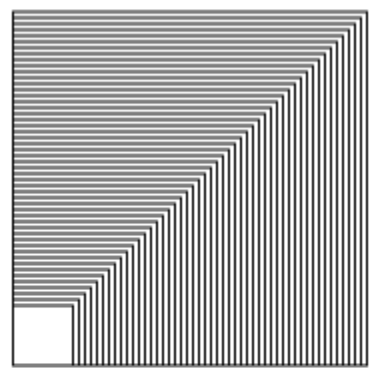
\includegraphics[width=\linewidth]{GrundlagenInfo/00_Programmieren/Figures/prog-8-squares.png}
    \end{figure}
\end{minipage}
\begin{table}[H]
    \centering
    \scriptsize
    \begin{tabular}{c|c}
         Variable & Wert \\\midrule
         \lstinline|aktuelle_seitenlaenge| & \lstinline|30|
    \end{tabular}
    \caption{Variablen-Tabelle für \pythoninline{quadrat_muster}}
    \label{tab:my_label}
\end{table}
\normalsize
\end{frame}